\documentclass{article}
\usepackage{ amssymb }
\usepackage{amsmath}
\usepackage{mathtools}
\usepackage{tikz}
\usepackage{multicol}
\usepackage{float}
\usepackage{graphicx}
\usepackage{subcaption}
\usepackage[margin=0.8in]{geometry}

\title{Numerical methods for Differential equations Report 1}
\author{Malte Wegener}
\date{September 2019}

\begin{document}

\maketitle
    
\section{Maxima of  2 Dimensional functions}
\subsection{a) Proof of Fermat's theorem}

A sufficiently smooth function $f(x)$ has a local maximum in $x_{0}$ if there exits $\delta > 0$ such that $f(x) \leq f(x_{0})$ for all $x, \mid x - x_{0} \mid > \delta$ \par
Therefore $f(x_{0}+\epsilon)-f(x_{0}) \leq 0$ for $\mid \epsilon \mid < \delta$
If we divide this by a small positive $\epsilon$, we get $\frac{f(x_{0}+\epsilon)-f(x_{0})}{\epsilon}\leq 0$.
Taking the limit as $\epsilon$ goes to 0, we get
\begin{equation*}
   \lim_{\epsilon\to 0^{+}} \frac{f(x_{0}+\epsilon)-f(x_{0})}{\epsilon}\leq 0
\end{equation*}

\begin{equation*}
   f'(x_{0})\leq 0
\end{equation*}

Similarly for $\epsilon < 0$

\begin{equation*}
   \lim_{\epsilon\to 0^{-}} \frac{f(x_{0}+\epsilon)-f(x_{0})}{\epsilon}\geq 0
  \end{equation*}
   
\begin{equation*}
   f'(x_{0})\geq 0
\end{equation*}

Thus $f'(x_{0}) = 0$

In order to seperate maxima from minima and saddle points, the second derivative has to be analysed.
Let $f(x)$ be a function with a maximum in $x=x_{0}$ that can be expanded by a taylor series around $x_{0}$. f in the neighborhood of $x_{0}$ can than be described by the following Taylor series.
\begin{equation*}
    f(x_{0}+\delta) = f(x_{0})+\delta*f'(x_{0})+\frac{\delta^2}{2}*f''(x_{0}) + \mathcal{O}(\delta^3)
\end{equation*}
As $f'(x_{0}) = 0$, as proven in a), This series can be rearranged for $f''(x_{0})$.

\begin{equation*}
    f(x_{0}+\delta) - f(x_{0}) = \frac{\delta^2}{2}*f''(x_{0}) + \mathcal{O}(\delta^3)
\end{equation*}
 As $f(x_{0}+\delta) - f(x_{0}) \leq 0$ in the neigborhood of $x_{0}$.
\begin{equation*}
    0 \geq \frac{\delta^2}{2}*f''(x_{0}) + \mathcal{O}(\delta^3)
\end{equation*}

Dividing by $\frac{\delta^2}{2}$.

\begin{equation*}
    0 \geq f''(x_{0}) + \mathcal{O}(\delta)
\end{equation*}

\begin{equation*}
    0 \geq \lim_{\delta \to 0} f''(x_{0}) + \mathcal{O}(\delta)
\end{equation*}

\begin{equation*}
    0 \geq f''(x_{0})
\end{equation*}

The derivative of a 2 dimensional function can be expressed as a vector pointing in the direction of the steepest direction uphill.
Let u be a be a sufficiently smooth function with a maximum in $ \left<x_{0}, y_{0}\right> $.$ u: \mathbb{R}^{2} \to \mathbb{R} $.
Let $f1(x) = u(x,y=y_{0})$ and $f2(y) = u(x=x_{0},y)$. Then
\begin{equation*}
    \frac{d}{dx}f1(x)\bigg|_{x=x_{0}} = 0 = \frac{\partial}{\partial x}f1(x)\bigg|_{x=x_{0},y=y_{0}}
\end{equation*}{}
\begin{equation*}
    \frac{d}{dy}f2(y)\bigg|_{y=y_{0}} = 0 = \frac{\partial}{\partial y}f2(y)\bigg|_{x=x_{0},y=y_{0}}
\end{equation*}{}

Thus $\nabla u = \mathbf{0}$

Similarly to the 1D case, the second derivative has to be analyzed. For this purposes the second derivative is defined as the Hessian of the function.
First the quadratic form of the Hessian is analyzed. Let $H$ be the Hessian matrix and $\mathbf{v}=\langle p, q\rangle$ a unit vector.
\begin{equation*}
 H = \begin{bmatrix}
      \frac{\partial^2 u}{\partial x^2} & \frac{\partial^2 u}{\partial xy}\\
      \frac{\partial^2 u}{\partial xy} & \frac{\partial^2 u}{\partial y^2}\\
    \end{bmatrix}
\end{equation*}

\begin{equation*}
\mathbf{v}^{T} H \mathbf{v}= p^2\frac{\partial^2 u}{\partial x^2}+(p+q)\frac{\partial^2 u}{\partial xy} +q^2\frac{\partial^2 u}{\partial x^2}
\end{equation*}

\begin{align*}
D_{\mathbf{v}}\left(D_{\mathbf{v}} u\right)=\mathbf{v}\cdot \nabla(\mathbf{v} \cdot \nabla u)=\mathbf{v}\cdot \nabla(p\frac{\partial u}{\partial x}+q\frac{\partial u}{\partial y})\\
D_{\mathbf{v}}\left(D_{\mathbf{v}} u\right)=p^2\frac{\partial^2 u}{\partial x^2}+(p+q)\frac{\partial^2 u}{\partial xy} +q^2\frac{\partial^2 u}{\partial x^2}
\end{align*}

Thus $\mathbf{v}^{T} H \mathbf{v}=D_{\mathbf{v}}\left(D_{\mathbf{v}} u\right)$.

% TODO LASt step i hate that step


\newpage
\section{Properties of the 1D negative Laplacian}
\subsection{a}
A domain $\Omega=\left[0,1\right]$ that is descretized as a uniform grid $\Omega_h$ with a uniform stepsize $h$, has $1/h+1$ grid points if 1 is an integer multiple of $h$. If it is not, however the last point of $\Omega_h$ is not on the boundary.
\begin{figure}[H]
\centering
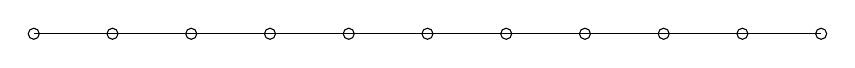
\begin{tikzpicture}
    \foreach \x in {0,...,10} 
        \draw (\x,3) circle (2pt);
    \draw (0,3) -- (10,3);
\end{tikzpicture}
\caption{$\Omega_h$}
\end{figure}

Let $\mathcal{L}=-\frac{d^{2}}{d x^{2}}$. Let u be discrete on a grid with a stepsize of $h$.
\begin{align}
    u_i &= u_i\\
    u_{i+1} &= u_i + h * u_i' + h^2/2 * u_i'' + h^3/6 * u_i''' + \mathcal{O}\left(h^4\right)\\
    u_{i-1} &= u_i - h * u_i' + h^2/2 * u_i'' - h^3/6 * u_i''' + \mathcal{O}\left(h^4\right)\\
\end{align}
\begin{align}
    D_x^+ &= \frac{u_{i+1}-u_i}{h} = u_i' + h/2 * u_i'' + h^2/6 * u_i''' + \mathcal{O}\left(h^3\right)\\
    D_x^- &= \frac{u_{i+1}-u_i}{h} = u_i' - h/2 * u_i'' + h^2/6 * u_i''' + \mathcal{O}\left(h^3\right)\\
    D_{xx} &= -1/h*\left(D_x^+ - D_x^-\right) = u_i'' + \mathcal{O}\left(h^2\right)\\
\end{align}
\begin{equation}
    \mathcal{L} \approx \frac{-u_{i-1}+2u_i-u_{i+1}}{h^2}
\end{equation}
This can be assembled in to a tridiagonal matrix $A$.
\begin{figure}[H]
    \centering
    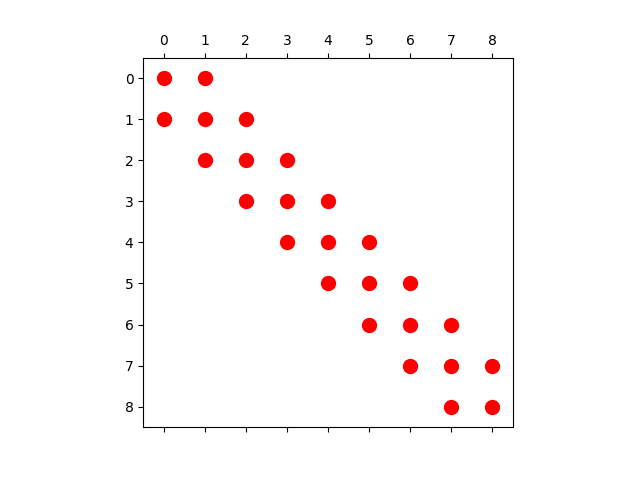
\includegraphics[width=.9\linewidth]{2spy.png}
    \caption{Structure of the Matrix $A$}
\end{figure}
As this matrix is small in size, the eigenvalues can be calculated numerically, as well as analytically. These eigenvalues can be compared to the first 9 eigenvalues of the Laplacian. It can be seen that the eigenvalues are very similar in the first eigenvalues but deviate significantly for later eigenvalues. Furthermore it can be seen that the eigenvalues are purely real.
\begin{figure}[H]
    \centering
    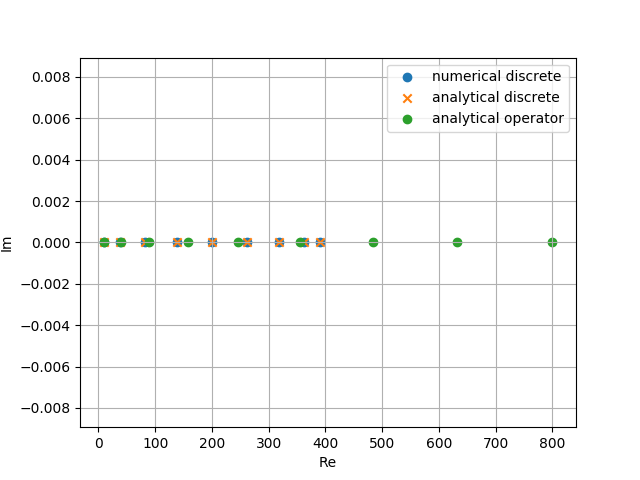
\includegraphics[width=.9\linewidth]{eigenvals.png}
    \caption{Eigenvalues of $A$ and $\mathcal{L}$}
\end{figure}
The corresponding eigenvectors can be plotted on the on the inner points of the domain together with the eigenfunctions of the Laplacian.
\begin{figure}[H]
    \centering
    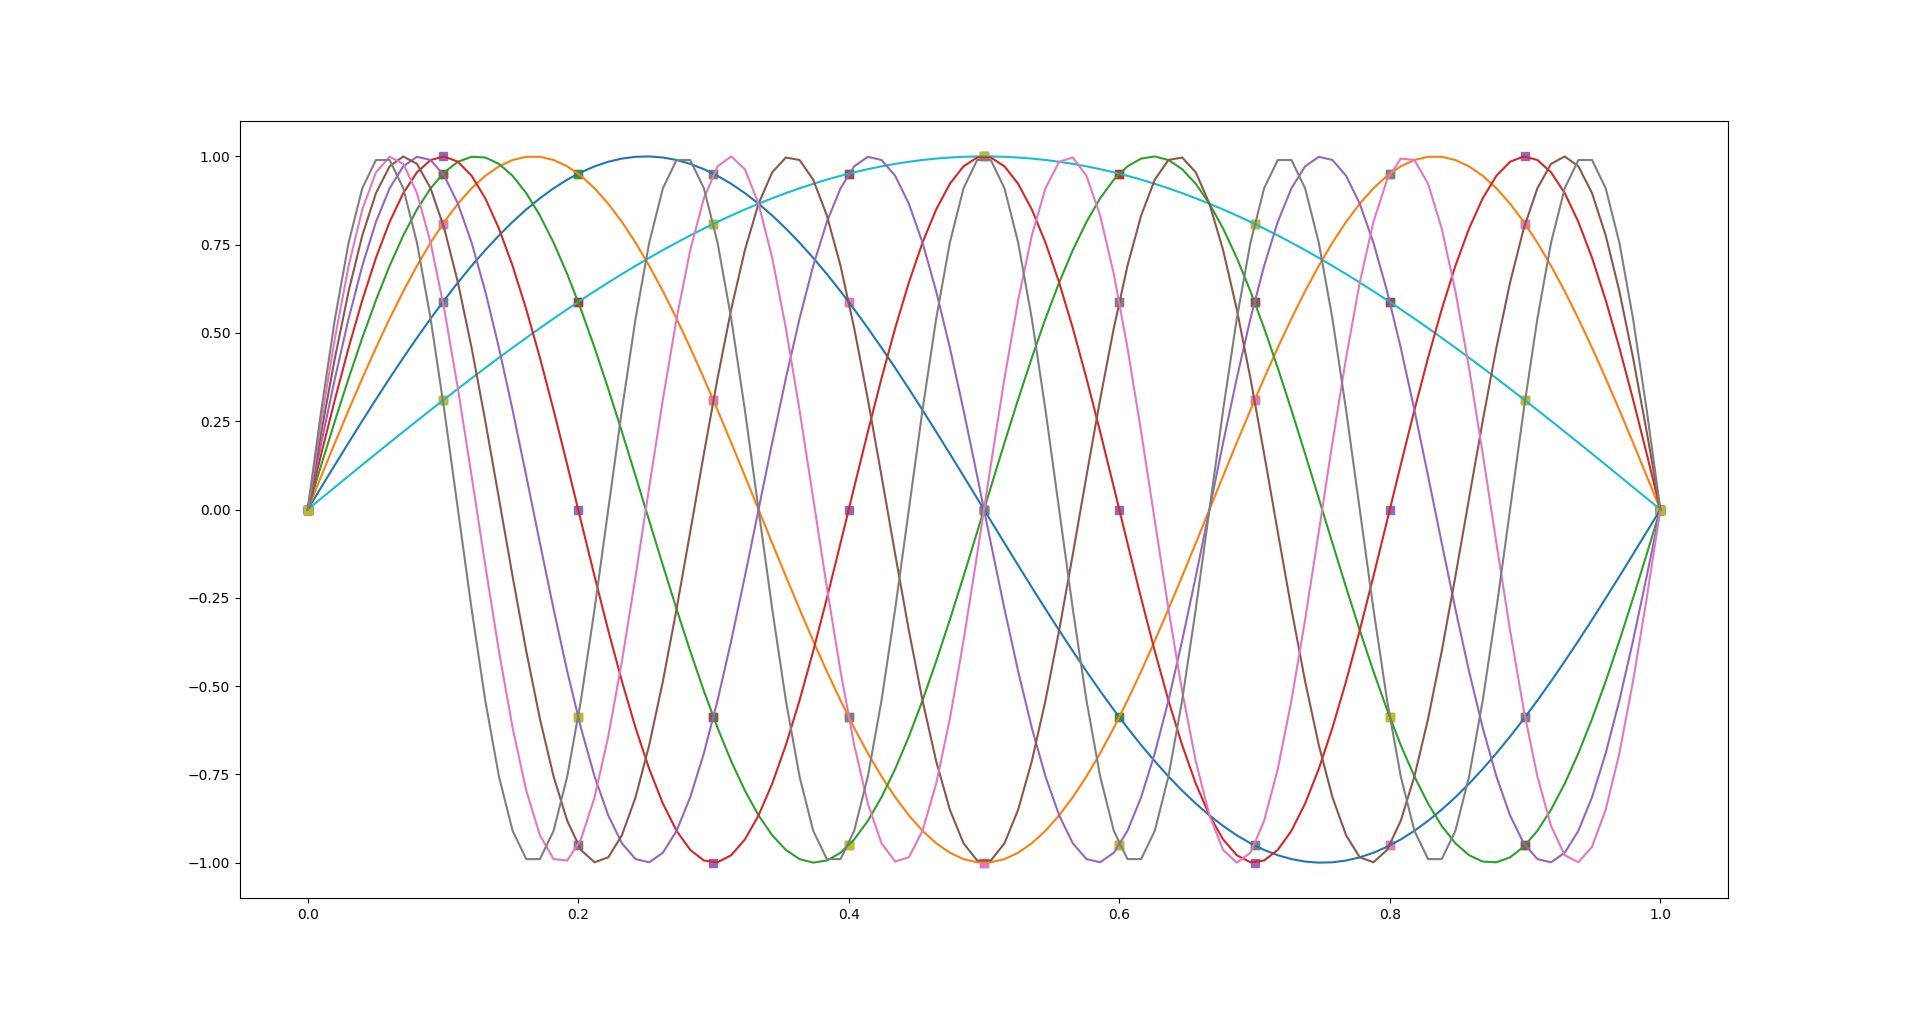
\includegraphics[width=.9\linewidth]{Eigenfuncs.png}
    \caption{Discrete eigenvectors (+) and continuous eigenfunctions}
\end{figure}

\section{1D boundary value problem}
Considering the following Boundary value problem, the solution can be found analytically.

\begin{align}
    -\frac{d^{2} u}{d x^{2}}=f_{i}, & x \in(0,1) \\ u(0)=1, & u(1)=2 \\ f_{1}(x)=1, \quad f_{2}(x)=e^{x}, & x \in[0,1]
\end{align}

\begin{align}
    -\frac{d^{2} u_1}{d x^{2}}=1 \\
    - d^2 u_1 = dx^2 \\
    - d u_1 = (x+C_1) dx\\
    - u_1 = \frac{1}{2}x^2 + C_1 x + C_2\\
    \text{with} u(0)=1,  u(1)=2 \\
    u_1 = -\frac{1}{2}x^2 - \frac{1}{2} x - 1\\
\end{align}

\begin{align}
    -\frac{d^{2} u_2}{d x^{2}}=e^x \\
    -d^2 u_2 = e^x dx^2 \\
    -d u_2 = (e^x+C_1) dx\\
    u_2 = -e^x + C_1 x + C_2\\
    \text{with} u(0)=1,  u(1)=2 \\
    u_2 = -e^x + e x + 2\\
\end{align}
In order to solve the given problem the second derivate has to be discretized on a grid with a stepsize of h. In the first step, h is chosen as $0.2$.

\begin{figure}[H]
    \centering
    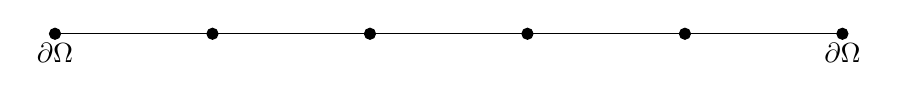
\begin{tikzpicture}
        \foreach \x in {1,...,4} 
            \filldraw (2*\x,5) circle (2pt);

        \filldraw (10,5) circle (2pt);
        \filldraw (0,5) circle (2pt);
        \draw (0,5) node[anchor=north] {$\partial \Omega$};
        \draw (10,5) node[anchor=north] {$\partial \Omega$};
        \draw (0,5) -- (10,5);
    \end{tikzpicture}
\end{figure}

\begin{align}
    u_i &= u_i\\
    u_{i+1} &= u_i + h * u_i' + h^2/2 * u_i'' + h^3/6 * u_i''' + \mathcal{O}\left(h^4\right)\\
    u_{i-1} &= u_i - h * u_i' + h^2/2 * u_i'' - h^3/6 * u_i''' + \mathcal{O}\left(h^4\right)\\
\end{align}
\begin{align}
    D_x^+ &= \frac{u_{i+1}-u_i}{h} = u_i' + h/2 * u_i'' + h^2/6 * u_i''' + \mathcal{O}\left(h^3\right)\\
    D_x^- &= \frac{u_{i+1}-u_i}{h} = u_i' - h/2 * u_i'' + h^2/6 * u_i''' + \mathcal{O}\left(h^3\right)\\
    D_{xx} &= -1/h*\left(D_x^+ - D_x^-\right) = u_i'' + \mathcal{O}\left(h^2\right)\\
\end{align}
\begin{equation}
    \mathcal{L} \approx \frac{-u_{i-1}+2u_i-u_{i+1}}{h^2}
\end{equation}
This can be assembled into a matrix similar to the one presented in section 2. With this matrix a system of linear equations can be assembled, where $\mathbf{u}$ is the discrete solution on of the problem on the inner rpoints of the domain. and $\mathbf{f}$ is the source function sampled on the inner points of the domain. The boundary conditions are applied in $\mathbf{b}$.
\begin{equation}
    A\mathbf{u} = \mathbf{f}+\mathbf{b}
\end{equation}
\begin{equation}
    \mathbf{b} = [u(0)/h^2, 0, \dots, 0, u(1)/h^2]^T\\
\end{equation}
Solving the linear system yields the following results
\begin{table}[H]
    \centering
    \begin{tabular}{c|c|c|c|c}
        & u1 numerical & u1 analytical & u2 numerical & u2 analytical \\ \hline
        0.2 & 1.28 & 1.28 & 1.3218 & 1.3223 \\ \hline
        0.4 & 1.52 & 1.52 & 1.5948 & 1.5954 \\ \hline
        0.6 & 1.72 & 1.72 & 1.8081 & 1.8089 \\ \hline
        0.8 & 1.88 & 1.88 & 1.0949 & 1.9490 \\ \hline
        L2 Error& $3.14 * 10^{-16}$ & N/A &0.00115 & N/A
        
    \end{tabular}
\end{table}

\begin{figure}[H]
    \begin{subfigure}{.5\textwidth}
      \centering
      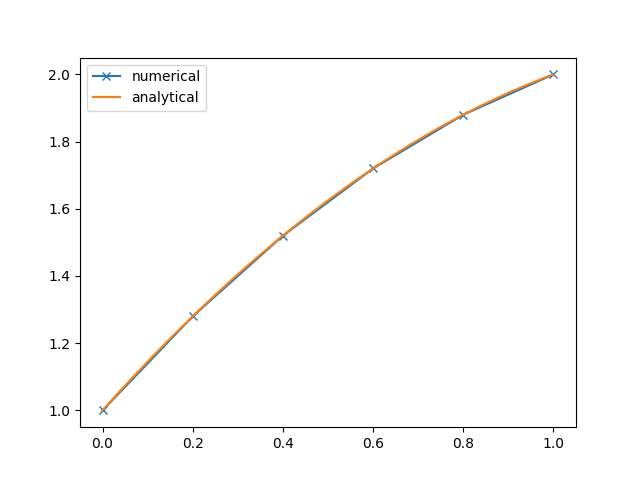
\includegraphics[width=.9\linewidth]{u1sym.png}
      \caption{Numerical and analytical solution of u1}
    \end{subfigure}%
    \begin{subfigure}{.5\textwidth}
      \centering
      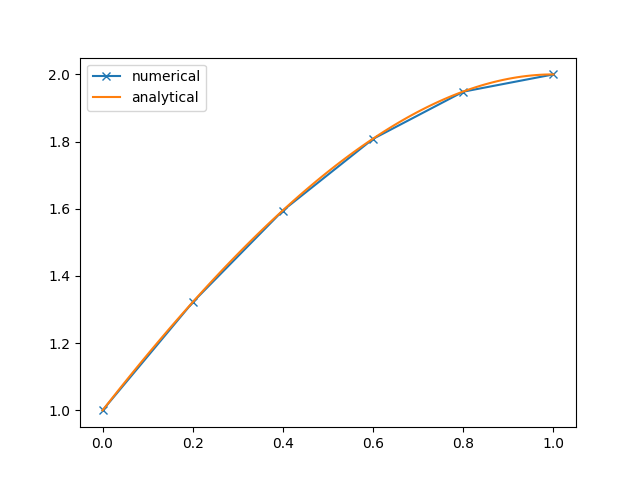
\includegraphics[width=.9\linewidth]{u2sym.png}
      \caption{Numerical and analytical solution of u2}
    \end{subfigure}
    \caption{Comparison of numerical and analytical solutions to the BVP}
\end{figure}
The domain can be refined by decreasing h. This will reduce the global error in the domain. By plotting the global error against the stepsize h, the rate of convergence can be seen. As this plot covers a high range of values, it is bettter to plot it on a double logarithmic plot, this also makes the plot appear linear. In order to understand the rate of convergence a logarithmic function of the form $f(x) = Ch^{\alpha}$. Fitting this function yields $\alpha=1.5$ and $C = 0.01278$. This indicates a rate of convergence between 1 and 2, as the Order of approximation is second order, this drop in convergence indicates the influence of the boudnary conditions.
\begin{figure}[H]
    \centering
    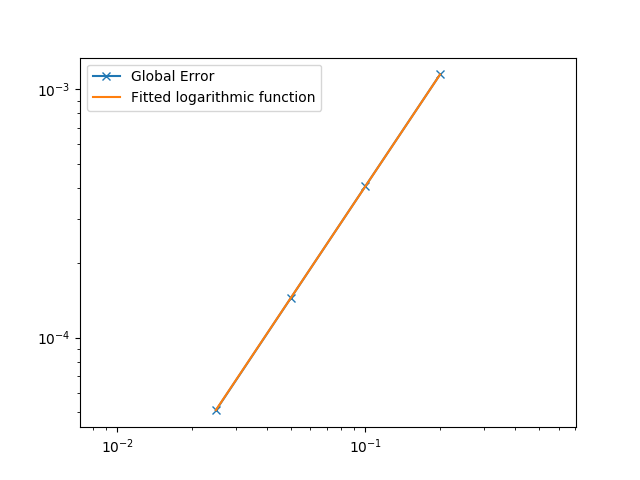
\includegraphics[width=.9\linewidth]{convergence.png}
    \caption{Convergence plot of the BVP}
\end{figure}


\section{4}
\newpage
\subsection{b}

    
Let $L$ be a discretized version of the Laplacian acting on a lexicographig vector of a 2 dimensional rectangular regular grid.
\begin{align}
    L\mathbf{u} &\approx \mathcal{L} u\\
    \mathcal{L} &= \frac{\partial^2}{\partial x^2} + \frac{\partial^2}{\partial x^2}
\end{align}

As $L$ is a linear operator, we can split it up into 2 seperate operators. Where $D_x'$ and $D_y'$ are the unknown versions of the discretized second derivative operators.

\begin{equation}
    L = D_x' + D_y'
\end{equation}

Lets consider a Matrix $M$.
\begin{equation}
    M = \begin{bmatrix}
        u_{1,1} & u_{1,2} & \dots & u_{1,n_y} \\
        u_{2,1} & u_{2,2} & \dots & u_{2,n_y} \\
        \vdots & \vdots & \ddots & \vdots \\
        u_{n_x,1} & u_{n_x,2} & \dots & u_{n_x,n_y}
    \end{bmatrix}
\end{equation}

Lets consider the discrete 1D versions of the Laplacian as $D_x$ and $D_y$, with sizes $n_x \times n_x$ and $n_y \times n_y$ respectively.
Let $M_x$ and $M_y$ be $nx\times ny$ matrices containing approximated second derivatives of $\mathbf{u}$ order similarly as in $M$. It than can easily proven that.
\begin{align}
    D_x M = M_x \\
    M D_y = M_y
\end{align}
Lets introduce $\operatorname{vec}(A)=\left[a_{1,1}, \ldots, a_{m, 1}, a_{1,2}, \ldots, a_{m, 2}, \ldots, a_{1, n}, \ldots, a_{m, n}\right]^{\mathrm{T}}$ as the vectorization of a Matrix. With this Operators, the following properties emerge.
\begin{align}
    \operatorname{vec}(M) &= \mathbf{u} \\
    \operatorname{vec}(M_x) + \operatorname{vec}(M_y) &= L\mathbf{u}
\end{align}
Using $\operatorname{vec}(A B)=\left(I_{m} \otimes A\right) \operatorname{vec}(B)=\left(B^{\mathrm{T}} \otimes I_{k}\right) \operatorname{vec}(A)$ and $D_y^{\mathrm{T}} = D_y$.
\begin{align}
    \operatorname{vec}(D_x M) = (I_{n_y} \otimes D_x)\operatorname{vec}(M) = \operatorname{vec}(M_x)\\
    \operatorname{vec}(M D_y) = (D_y \otimes I_{n_x})\operatorname{vec}(M) = \operatorname{vec}(M_y)
\end{align} 
As $\operatorname{vec}(M) = \mathbf{u}$, $D_x' \mathbf{u} = \operatorname{vec}(M_x)$ and $D_y' \mathbf{u} = \operatorname{vec}(M_y)$.
\begin{align}
    (I_{n_y} \otimes D_x) = D_x' \\
    (D_y \otimes I_{n_x}) = D_y'
\end{align}
Thus $(I_{n_y} \otimes D_x) + (D_y \otimes I_{n_x}) = L$


In order to apply the Dirichlet Boundary Conditions, a vector $\mathbf{b}$ has to be added to the right hand side of the System. Let the Boundaries of th domain be denoted by North, West, South and East with their functions $f_N, f_W, f_S, f_E$ respectively. Let $b_N = \left[f_N(h_x), f_N(h_x*2), \dots, f_N(h_x*n_x\right]$ % TODO Add other Vectors Ugh
Let $\mathbf{e}_{m,n}$ denote a unitvector of length m with a 1 in the n\textsuperscript{th} postion.
Then $\mathbf{b} = \mathbf{e}_{n_y,1} \otimes \mathbf{b}_S + \mathbf{e}_{n_y,n_y} \otimes \mathbf{b}_S + \mathbf{b}_W \otimes \mathbf{e}_{n_x,1} + \mathbf{b}_E \otimes \mathbf{e}_{n_x,n_x}$.

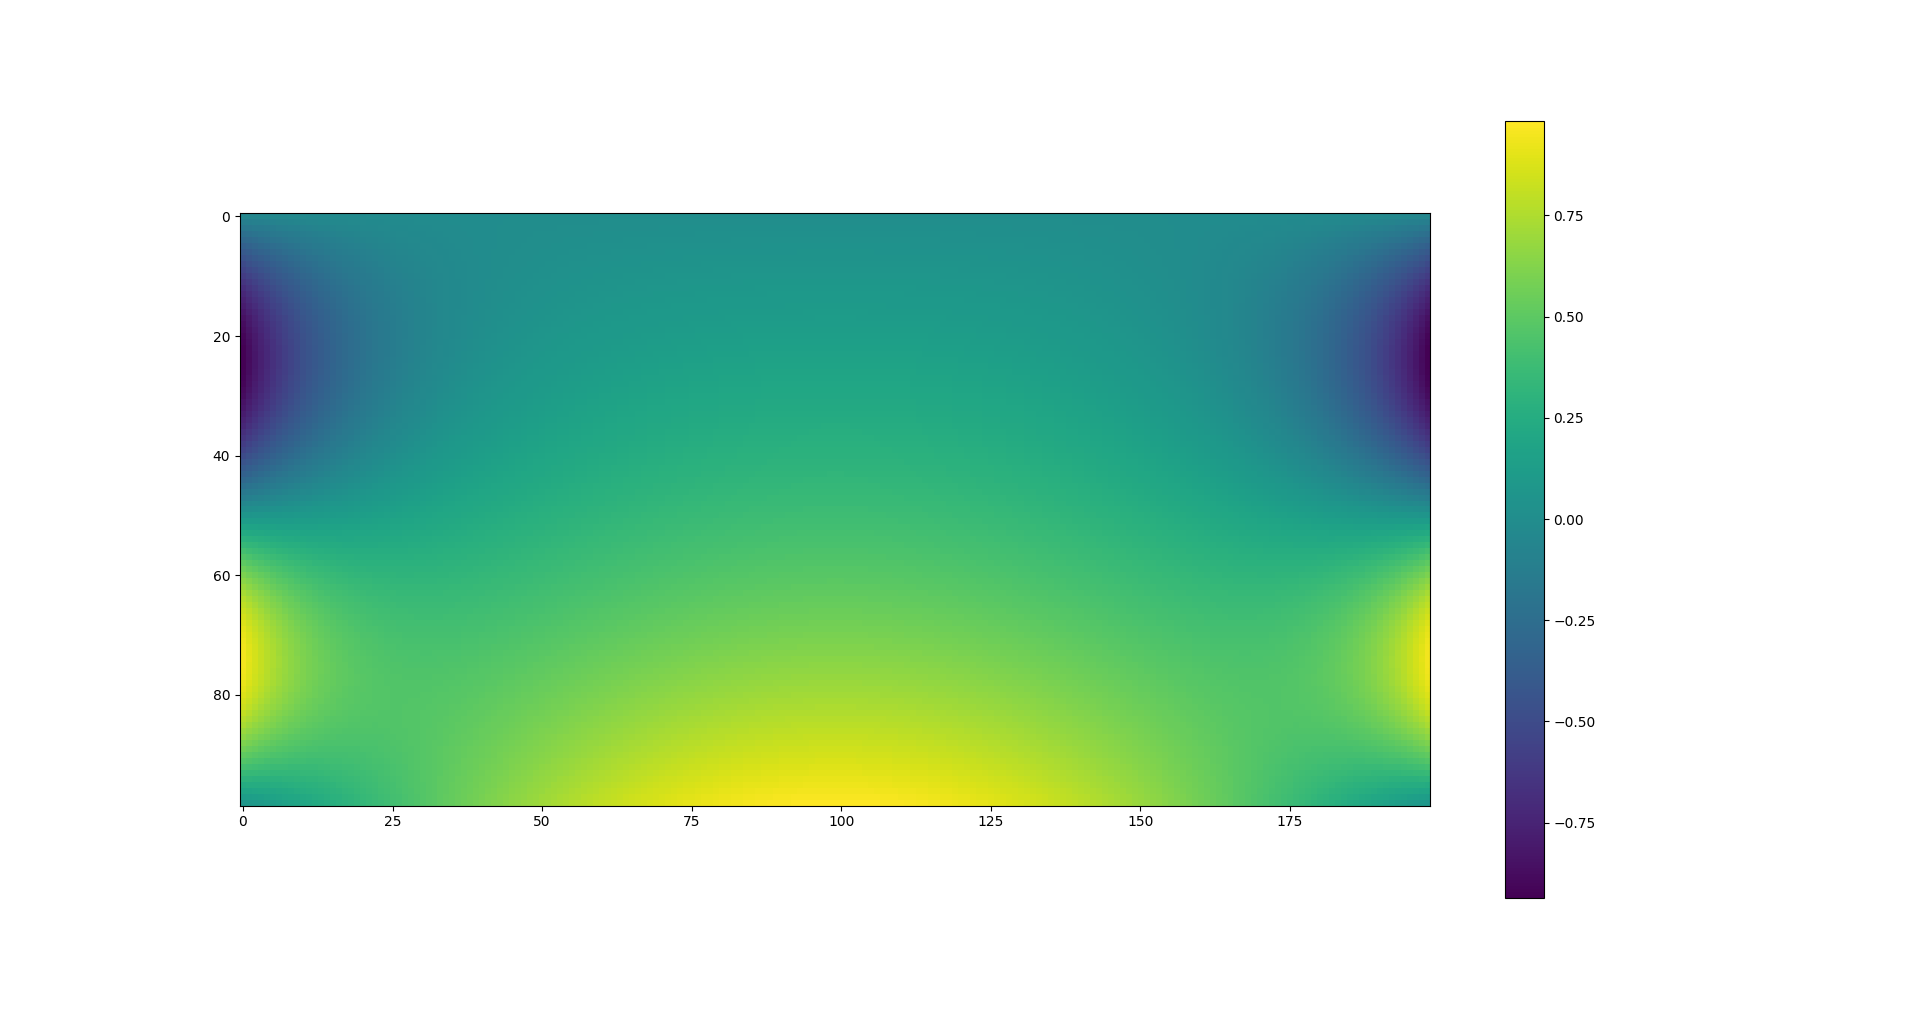
\includegraphics[width=\linewidth]{Figure_1.png}

%\end{multicols}
\end{document}